
%%--------------------------------------------------
%% CPO: Multiple Choice Questions
%%--------------------------------------------------


%% Chapter 6: Systems in Motion
%%--------------------------------------------------


%% Learning Objectives
%%--------------------------------------------------

%% Define projectile. 
%% Recognize the independence of a projectile’s horizontal and vertical velocities. 
%% Describe the path of a projectile.
%% Calculate a projectile’s horizontal and vertical velocities. 
%% Explain how a projectile’s launch angle affects its range. 
%% Distinguish between rotation and revolution. 
%% Calculate angular speed. 
%% Explain how angular speed, linear speed, and distance are related. 
%% Explain how centripetal force causes circular motion. 
%% List the factors that affect centripetal force. 
%% Describe the relationship between gravitational force, mass, and distance. 
%% Relate centripetal force to orbital motion. 
%% Define center of mass and center of gravity. 
%% Explain how to locate an object’s center of mass and center of gravity. 
%% Use the concept of center of gravity to explain toppling.


%% CPO Multiple Choice Questions
%%--------------------------------------------------
\element{cpo-mc}{
\begin{question}{cpo-ch06-q01}
    The parabolic path followed by a projectile is referred to as the:
    \begin{multicols}{2}
    \begin{choices}
        \wrongchoice{range}
      \correctchoice{trajectory}
        \wrongchoice{circumference}
        \wrongchoice{ellipse}
    \end{choices}
    \end{multicols}
\end{question}
}

\element{cpo-mc}{
\begin{question}{cpo-ch06-q02}
    A golf ball will have the greatest range when it is hit with respect to the horizontal at an angle of:
    \begin{multicols}{2}
    \begin{choices}
        \wrongchoice{\ang{30}}
      \correctchoice{\ang{45}}
        \wrongchoice{\ang{60}}
        \wrongchoice{\ang{90}}
    \end{choices}
    \end{multicols}
\end{question}
}

\element{cpo-mc}{
\begin{questionmult}{cpo-ch06-Q03}
    The distance a projectile travels is dependent upon:
    \begin{multicols}{2}
    \begin{choices}
      \correctchoice{air resistance}
      \correctchoice{launch angle}
      \correctchoice{launch speed}
      \correctchoice{gravitational acceleration}
      \correctchoice{initial height}
    \end{choices}
    \end{multicols}
\end{questionmult}
}

\element{cpo-mc}{
\begin{question}{cpo-ch06-q04}
    The distance a projectile travels horizontally in the air may be called its:
    \begin{multicols}{2}
    \begin{choices}
        \wrongchoice{trajectory}
      \correctchoice{range}
        \wrongchoice{parabola}
        \wrongchoice{height}
    \end{choices}
    \end{multicols}
\end{question}
}

\element{cpo-mc}{
\begin{question}{cpo-ch06-q05}
    If a ball thrown horizontally with a speed of \SI{15}{\meter\per\second} travels for \SI{5}{\second} before hitting the ground,
        its range after \SI{4}{\second} would be:
    \begin{multicols}{2}
    \begin{choices}
        \wrongchoice{\SI{15}{\meter}}
        \wrongchoice{\SI{39}{\meter}}
      \correctchoice{\SI{60}{\meter}}
        \wrongchoice{\SI{153}{\meter}}
    \end{choices}
    \end{multicols}
\end{question}
}

\element{cpo-mc}{
\begin{question}{cpo-ch06-q06}   
    Of the following, the one that would \emph{not} be considered a projectile is a:
    \begin{choices}
      \correctchoice{crow flying between trees.}
        \wrongchoice{football thrown by a high school quarterback.}
        \wrongchoice{tennis ball hit by a star tennis player.}
        \wrongchoice{fox jumping over a wall.}
    \end{choices}
\end{question}
}

\element{cpo-mc}{
\begin{question}{cpo-ch06-q07}
    Jennifer and Tamar throw a snowball at the same time horizontally from a height of \SI{1.5}{\meter}.
    Jennifer throws hers at a speed of \SI{6.0}{\meter\per\second}.
    If Tamar throws hers at \SI{12}{\meter\per\second},
        her snowball will:
    \begin{choices}
        \wrongchoice{travel the same distance as Jennifer's before hitting the ground.}
        \wrongchoice{hit the ground later than Jennifer's.}
        \wrongchoice{travel half the distance as Jennifer's before hitting the ground.}
      \correctchoice{hit the ground at the same time as Jennifer's.}
    \end{choices}
\end{question}
}

\element{cpo-mc}{
\begin{question}{cpo-ch06-q08}
    The golf ball that will travel farthest is one hit at an angle of:
    \begin{multicols}{2}
    \begin{choices}
        \wrongchoice{\ang{20}}
        \wrongchoice{\ang{30}}
        \wrongchoice{\ang{40}}
      \correctchoice{\ang{60}}
    \end{choices}
    \end{multicols}
\end{question}
}

\element{cpo-mc}{
\begin{question}{cpo-ch06-q09}
    If a ball thrown horizontally with a speed of \SI{15}{\meter\per\second} travels for \SI{5}{\second} before hitting the ground,
        its horizontal speed after \SI{4}{\second} is:
    \begin{multicols}{2}
    \begin{choices}
      \correctchoice{\SI{15}{\meter\per\second}}
        \wrongchoice{\SI{39}{\meter\per\second}}
        \wrongchoice{\SI{60}{\meter\per\second}}
        \wrongchoice{\SI{75}{\meter\per\second}}
    \end{choices}
    \end{multicols}
\end{question}
}

\element{cpo-mc}{
\begin{question}{cpo-ch06-q10}
    A stunt car driver traveling at \SI{30}{\meter\per\second} drives his car off a \SI{20}{\meter} high cliff as illustrated in the diagram:
    \begin{center}
    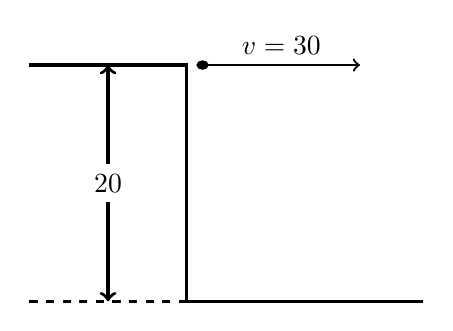
\begin{tikzpicture}[yscale=0.75]
        \draw[very thick] (-2,0) -- (0,0) -- (0,-4) -- (3,-4);
        \draw[fill] (0.2,0.0) circle [radius=2pt];
        \draw[thick,->] (0.2,0.0) -- ++ (0:2)
            node[pos=0.5,anchor=south] {$v=\SI{30}{\meter\per\second}$};
        \draw[very thick,dashed] (-2,-4) -- (0,-4);
        \node (A) at (-1,-2.0) {\SI{20}{\meter}};
        \draw[very thick,->] (A) -- (-1,0);
        \draw[very thick,->] (A) -- (-1,-4);
    \end{tikzpicture}
    \end{center}
    How far from the base of the cliff does the car hit?
    \begin{multicols}{2}
    \begin{choices}
        \wrongchoice{\SI{41}{\meter}}
      \correctchoice{\SI{61}{\meter}}
        \wrongchoice{\SI{82}{\meter}}
        \wrongchoice{\SI{122}{\meter}}
    \end{choices}
    \end{multicols}
\end{question}
}

\element{cpo-mc}{
\begin{question}{cpo-ch06-q11}
    A soccer ball is kicked into the air with an initial vertical velocity of \SI{+49}{\meter\per\second} and a horizontal velocity of \SI{19.6}{\meter\per\second}.
    The diagram representing the vertical and horizontal velocity of the balls after \SI{2}{\second} of flight is:
    [Vectors are drawn to scale]
    \begin{multicols}{2}
    \begin{choices}
        \AMCboxDimensions{down=-1em}
        \wrongchoice{
            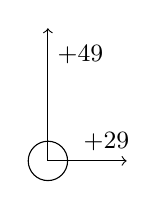
\begin{tikzpicture}[scale=0.5,font=\small]
                %% To make each same size 
                \draw[white] (0,0) (0,3.37);
                %% Draw ball with velocity vectors
                \draw (0,0) circle (0.5);
                \draw[->] (0,0) -- ++(0:2)
                    node[pos=0.33,anchor=south west] {\SI{+29}{\meter\per\second}};
                \draw[->] (0,0) -- ++(90:3.37)
                    node[pos=0.66,anchor=south west] {\SI{+49}{\meter\per\second}};
            \end{tikzpicture}
        }
        \wrongchoice{
            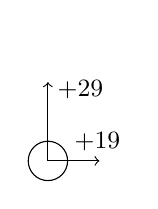
\begin{tikzpicture}[scale=0.5,font=\small]
                \draw[white] (0,0) (0,3.37);
                \draw (0,0) circle (0.5);
                \draw[->] (0,0) -- ++(0:1.31)
                    node[pos=0.33,anchor=south west] {\SI{+19}{\meter\per\second}};
                \draw[->] (0,0) -- ++(90:2)
                    node[pos=0.66,anchor=south west] {\SI{+29}{\meter\per\second}};
            \end{tikzpicture}
        }
        \wrongchoice{
            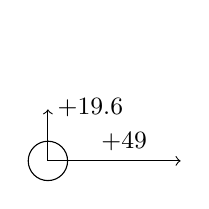
\begin{tikzpicture}[scale=0.5,font=\small]
                \draw[white] (0,0) (0,3.37);
                \draw (0,0) circle (0.5);
                \draw[->] (0,0) -- ++(0:3.37)
                    node[pos=0.33,anchor=south west] {\SI{+49}{\meter\per\second}};
                \draw[->] (0,0) -- ++(90:1.31)
                    node[pos=0.66,anchor=south west] {\SI{+19.6}{\meter\per\second}};
            \end{tikzpicture}
        }
        \wrongchoice{
            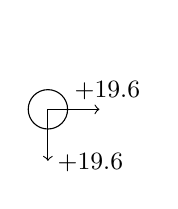
\begin{tikzpicture}[scale=0.5,font=\small]
                \draw[white] (0,0) (0,2.06);
                \draw (0,0) circle (0.5);
                \draw[->] (0,0) -- ++(0:1.31)
                    node[pos=0.33,anchor=south west] {\SI{+19.6}{\meter\per\second}};
                \draw[->] (0,0) -- ++(-90:1.31)
                    node[pos=0.66,anchor=north west] {\SI{+19.6}{\meter\per\second}};
            \end{tikzpicture}
        }
    \end{choices}
    \end{multicols}
\end{question}
}

\element{cpo-mc}{
\begin{question}{cpo-ch06-q12}   
    A water balloon leaves a launcher at a certain speed and travels \SI{125}{yards} when launched at an angle of \ang{23} to the ground.
    If launched at the same speed, it would travel the same distance when launched at angle of:
    \begin{multicols}{4}
    \begin{choices}
        \wrongchoice{\ang{22}}
        \wrongchoice{\ang{46}}
      \correctchoice{\ang{67}}
        \wrongchoice{\ang{77}}
    \end{choices}
    \end{multicols}
\end{question}
}

\element{cpo-mc}{
\begin{question}{cpo-ch06-q13}
    A projectile launched at a speed of \SI{35}{\meter\per\second} will have the greatest horizontal speed when launched at an angle of:
    \begin{multicols}{4}
    \begin{choices}
        \wrongchoice{\ang{20}}
        \wrongchoice{\ang{30}}
      \correctchoice{\ang{45}}
        \wrongchoice{\ang{60}}
    \end{choices}
    \end{multicols}
\end{question}
}

\element{cpo-mc}{
\begin{question}{cpo-ch06-q14}
    Angular speed can measure:
    \begin{choices}
        \wrongchoice{the rate at which an object moves in a straight line.}
        \wrongchoice{the rate at which an object revolves around an external axis.}
        \wrongchoice{the rate at which an object rotates around an external axis.}
      \correctchoice{both the rate of rotating and revolving.}
    \end{choices}
\end{question}
}

\element{cpo-mc}{
\begin{question}{cpo-ch06-q15}
    An example of rotation is:
    \begin{choices}
        \wrongchoice{Earth moving in its orbit around the sun.}
      \correctchoice{a basketball spinning on the end of a finger.}
        \wrongchoice{a race car traveling at \SI{200}{\mile\per\hour} around a circular track.}
        \wrongchoice{a student riding at the outside position on a merry-go-round.}
    \end{choices}
\end{question}
}

\element{cpo-mc}{
\begin{question}{cpo-ch06-q16}
    Mao watches a merry-go-round as it turns 27 times in \SI{3}{\minute}.
    The angular speed of the merry-go-round is:
    \begin{multicols}{2}
    \begin{choices}
        %% NOTE: radians per minute or second??
        \wrongchoice{\SI{81}{rpm}}
        \wrongchoice{\SI{27}{rpm}}
      \correctchoice{\SI{90}{rpm}}
        \wrongchoice{\SI{0.11}{rpm}}
    \end{choices}
    \end{multicols}
\end{question}
}

\element{cpo-mc}{
\begin{question}{cpo-ch06-q17}
    Three students are seated on a merry-go-round.
    Randy is seated closest to the center, Toby is seated near the outer edge, and Rasheed is seated between them.
    As the merry-go-round turns:
    \begin{choices}
        \wrongchoice{Randy has the greatest linear speed but the lowest angular speed.}
      \correctchoice{Toby has the highest linear speed but the lowest angular speed.}
        \wrongchoice{Rasheed has the same linear speed as the others but the highest angular speed.}
        \wrongchoice{All three students have the same linear and angular speed.}
    \end{choices}
\end{question}
}

\element{cpo-mc}{
\begin{question}{cpo-ch06-q18}
    Anika twirls a ball on a string which is \SI{3}{\meter} long.
    If the ball makes 2 revolutions per second,
        the linear speed of the ball is about:
    \begin{multicols}{2}
    \begin{choices}
        \wrongchoice{\SI{6}{\meter\per\second}}
        \wrongchoice{\SI{10}{\meter\per\second}}
        \wrongchoice{\SI{19}{\meter\per\second}}
      \correctchoice{\SI{38}{\meter\per\second}}
    \end{choices}
    \end{multicols}
\end{question}
}

\element{cpo-mc}{
\begin{question}{cpo-ch06-q19}
    Spiderman swings on the end of a web that is \SI{20}{\meter} long in an arc of \ang{45} to get from one building to another.
    The trip takes him \SI{5.0}{\second}.
    Spiderman travels from building to building at a linear speed of:
    \begin{multicols}{2}
    \begin{choices}
        \wrongchoice{\SI{2.0}{\meter\per\second}}
        \wrongchoice{\SI{6.3}{\meter\per\second}}
      \correctchoice{\SI{10}{\meter\per\second}}
        \wrongchoice{\SI{31}{\meter\per\second}}
    \end{choices}
    \end{multicols}
\end{question}
}

\element{cpo-mc}{
\begin{question}{cpo-ch06-q20}
    A record rotating at 33 rotations per minute has an angular speed of:
    \begin{multicols}{2}
    \begin{choices}
        \wrongchoice{\SI{33}{\degree\per\minute}}
        \wrongchoice{\SI{55}{\degree\per\second}}
      \correctchoice{\SI{198}{\degree\per\second}}
        \wrongchoice{\SI{55}{\degree\per\minute}}
    \end{choices}
    \end{multicols}
\end{question}
}

\element{cpo-mc}{
\begin{question}{cpo-ch06-q21}
    Erica pedals her bicycle from home to a local store \SI{2.5}{\mile} away.
    The wheels on Erica's bicycle have a diameter of \SI{27}{\inch}.
    The number of revolutions made by the wheels of her bicycle on this ride is:
    \begin{multicols}{2}
    \begin{choices}
        \wrongchoice{\num{1 100}.}
      \correctchoice{\num{1 900}.}
        \wrongchoice{\num{13 000}.}
        \wrongchoice{\num{22 000}.}
    \end{choices}
    \end{multicols}
\end{question}
}

\element{cpo-mc}{
\begin{question}{cpo-ch06-q22}
    The speedometer on a bicycle registers speed by converting angular speed of a bicycle's wheel to linear speed.
    What is the approximate speed that would be indicated by the speedometer of a bicycle wheel with a diameter of \SI{0.70}{\meter} rotating at a rate of 3 rotations per second?
    \begin{multicols}{2}
    \begin{choices}
        \wrongchoice{\SI{2.2}{\meter\per\second}.}
        \wrongchoice{\SI{4.3}{\meter\per\second}.}
      \correctchoice{\SI{6.6}{\meter\per\second}.}
        \wrongchoice{\SI{21}{\meter\per\second}.}
    \end{choices}
    \end{multicols}
\end{question}
}

\element{cpo-mc}{
\begin{question}{cpo-ch06-q23}
    Any force that causes an object to move in a circle is called a \rule[-0.1pt]{4em}{0.1pt} force.
    \begin{multicols}{2}
    \begin{choices}
        \wrongchoice{gravitational}
      \correctchoice{centripetal}
        \wrongchoice{linear}
        \wrongchoice{frictional}
    \end{choices}
    \end{multicols}
\end{question}
}

\element{cpo-mc}{
\begin{question}{cpo-ch06-q24}
    The source of the centripetal force that allows a race car to go around a corner is:
    \begin{multicols}{2}
    \begin{choices}
        \wrongchoice{gravity}
      \correctchoice{friction}
        \wrongchoice{inertia}
        \wrongchoice{momentum}
    \end{choices}
    \end{multicols}
\end{question}
}

\element{cpo-mc}{
\begin{question}{cpo-ch06-q25}
    The weight of an automobile depends upon all of the following factors \emph{except} the:
    \begin{choices}
      \correctchoice{speed of the automobile on the road.}
        \wrongchoice{mass of the earth.}
        \wrongchoice{mass of the automobile.}
        \wrongchoice{distance of the automobile from Earth's center.}
    \end{choices}
\end{question}
}

\element{cpo-mc}{
\begin{question}{cpo-ch06-q26}
    You cannot feel a gravitational force acting between you and a friend because:
    \begin{choices}
        \wrongchoice{gravity is a force applied only by Earth.}
        \wrongchoice{living things do not exert any gravitational force.}
      \correctchoice{the mass of a person is not large enough to exert gravitational force that can be felt.}
        \wrongchoice{the distance between attracting objects must be very large for gravity to act.}
    \end{choices}
\end{question}
}

\element{cpo-mc}{
\begin{question}{cpo-ch06-q27}
    The path followed by one object as it revolves around another is called its:
    \begin{multicols}{2}
    \begin{choices}
        \wrongchoice{trajectory}
      \correctchoice{orbit}
        \wrongchoice{satellite}
        \wrongchoice{center of mass}
    \end{choices}
    \end{multicols}
\end{question}
}

\element{cpo-mc}{
\begin{question}{cpo-ch06-q28}
    Factors that affect the amount of centripetal force on an object moving in a circle include all of the following \emph{except}:
    %% NOTE: this was wrong in document
    \begin{choices}
        \wrongchoice{speed of the object}
        \wrongchoice{radius of revolution}
        \wrongchoice{mass of the object}
      \correctchoice{direction of motion (clockwise of counterclockwise)}
    \end{choices}
\end{question}
}

\element{cpo-mc}{
\begin{question}{cpo-ch06-q29}
    All of the following represent objects that are being accelerated \emph{except} a:
    \begin{choices}
        \wrongchoice{car moving around a corner at a constant speed of \SI{30}{\mile\per\hour}.}
        \wrongchoice{competitor in a track meet increasing speed at the finish line to pass another runner.}
      \correctchoice{bird flying in a straight line from one tree to another at high speed.}
        \wrongchoice{jet airliner banking into a turn as it slows to prepare for a landing.}
    \end{choices}
\end{question}
}

\element{cpo-mc}{
\begin{question}{cpo-ch06-q30}
    According to the diagram, the direction of the centripetal force on the airplane is directed toward:
    \begin{center}
    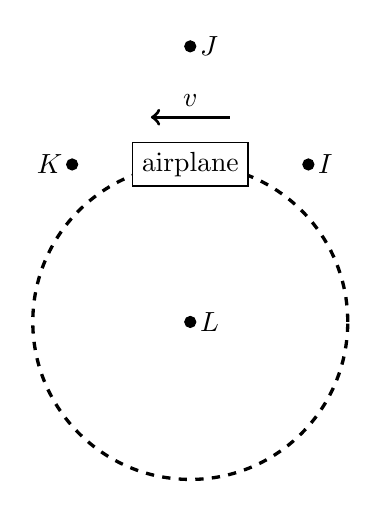
\begin{tikzpicture}
        \draw[very thick,dashed] (0,0) circle (2cm);
        \node[draw,fill=white,rectangle,minimum width=3em,minimum height=1em] (P) at (90:2cm) {airplane};
        \draw[very thick,->] (0.5cm,2.6cm) -- (-0.5cm,2.6cm)
            node[pos=0.5,anchor=south] {$v$};
        \draw[fill] (P) ++(0:1.5cm) circle (2pt)
            node[anchor=west] {$I$};
        \draw[fill] (P) ++(90:1.5cm) circle (2pt)
            node[anchor=west] {$J$};
        \draw[fill] (P) ++(180:1.5cm) circle (2pt)
            node[anchor=east] {$K$};
        \draw[fill] (0,0) circle (2pt)
            node[anchor=west] {$L$};
    \end{tikzpicture}
    \end{center}
    \begin{multicols}{4}
    \begin{choices}
        \wrongchoice{$I$}
        \wrongchoice{$J$}
        \wrongchoice{$K$}
      \correctchoice{$L$}
    \end{choices}
    \end{multicols}
\end{question}
}

\element{cpo-mc}{
\begin{question}{cpo-ch06-q31}
    If you climb a hill, you are farther from the center of Earth.
    Due to your new location, your weight will:
    \begin{choices}
      \correctchoice{decrease by a tiny amount.}
        \wrongchoice{decrease by a large amount.}
        \wrongchoice{increase by a tiny amount.}
        \wrongchoice{increase by a large amount.}
    \end{choices}
\end{question}
}

\element{cpo-mc}{
\begin{question}{cpo-ch06-q32}
    The factor that will \emph{increase} your weight the \emph{most} is:
    \begin{choices}
      \correctchoice{doubling your mass.}
        \wrongchoice{halving your mass.}
        \wrongchoice{doubling your distance from the Earth's center.}
        \wrongchoice{halving your distance from the Earth's center.}
    \end{choices}
\end{question}
}

\element{cpo-mc}{
\begin{question}{cpo-ch06-q33}
    If the radius of the curve around which a car is driven is increased,
        the following can be said about the centripetal force required to cause the car to go around the corner at constant speed:
    \begin{choices}
        \wrongchoice{The centripetal force increases.}
      \correctchoice{The centripetal force decreases.}
        \wrongchoice{The centripetal force remains the same.}
        \wrongchoice{There is insufficient information to make a determination about the centripetal force.}
    \end{choices}
\end{question}
}

\element{cpo-mc}{
\begin{question}{cpo-ch06-q34}
    A ball is being twirled on the end of a string as pictured in the diagram:
    \begin{center}
    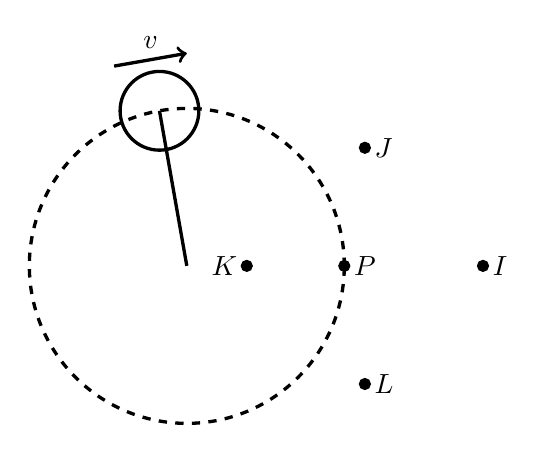
\begin{tikzpicture}
        \draw[very thick,dashed] (0,0) circle (2cm);
        \draw[very thick] (0,0) -- (100:2cm) circle (0.5cm);
        \draw[very thick,->] (110:2.7cm) -- (90:2.7cm)
            node[pos=0.5,anchor=south] {$v$};
        \draw[fill] (0:2cm) circle (2pt)
            node[anchor=west] (P) {$P$};
        \draw[fill] (P) ++(0:1.5cm) circle (2pt)
            node[anchor=west] {$I$};
        \draw[fill] (P) ++(90:1.5cm) circle (2pt)
            node[anchor=west] {$J$};
        \draw[fill] (P) ++(180:1.5cm) circle (2pt)
            node[anchor=east] {$K$};
        \draw[fill] (P) ++(270:1.5cm) circle (2pt)
            node[anchor=west] {$L$};
    \end{tikzpicture}
    \end{center}
    If the string is released when the ball reaches point $P$,
        the inertia of the ball will cause it to move in the direction of:
    \begin{multicols}{4}
    \begin{choices}
        \wrongchoice{$I$}
        \wrongchoice{$J$}
        \wrongchoice{$K$}
      \correctchoice{$L$}
    \end{choices}
    \end{multicols}
\end{question}
}

\element{cpo-mc}{
\begin{question}{cpo-ch06-q35}
    The centripetal force on a \SI{20}{\kilo\gram} object revolving on the end of a \SI{10}{\meter} long cord is \SI{20}{\newton}.
    If the linear speed of the object is doubled, the centripetal force required to keep it moving in a circle of the same radius is: 
    \begin{multicols}{2}
    \begin{choices}
        \wrongchoice{\SI{10}{\newton}}
        \wrongchoice{\SI{40}{\newton}}
      \correctchoice{\SI{80}{\newton}}
        \wrongchoice{\SI{200}{\newton}}
    \end{choices}
    \end{multicols}
\end{question}
}

\element{cpo-mc}{
\begin{question}{cpo-ch06-q36}
    Examples of centripetal force include all of the following \emph{except}:
    \begin{choices}
        \wrongchoice{gravity of the sun acting to keep Earth in orbit.}
        \wrongchoice{the door of a car pushing on a passenger as the car rounds a corner.}
      \correctchoice{The friction between a dragster and the track as the car accelerates down the drag strip.}
        \wrongchoice{The force of the air pushing on the wings of a plane as it makes a turn.}
    \end{choices}
\end{question}
}

\element{cpo-mc}{
\begin{question}{cpo-ch06-q37}
    The force required to keep an object moving in a circle of the same radius while its mass is doubled and its speed is reduced to half would be:
    \begin{multicols}{2}
    \begin{choices}
        \wrongchoice{the same}
        \wrongchoice{doubled}
      \correctchoice{halved}
        \wrongchoice{quadrupled}
    \end{choices}
    \end{multicols}
\end{question}
}

\element{cpo-mc}{
\begin{question}{cpo-ch06-q38}
    If the distance between two objects is doubled while the masses of both objects are doubled,
        the gravitational force between then is
    \begin{multicols}{2}
    \begin{choices}
        \wrongchoice{halved}
      \correctchoice{the same}
        \wrongchoice{doubled}
        \wrongchoice{quadrupled}
    \end{choices}
    \end{multicols}
\end{question}
}

\element{cpo-mc}{
\begin{question}{cpo-ch06-q39}
    The mass of the planet Jupiter is \num{318} times greater than Earth's mass,
        and its radius is \num{11.2} times greater than that of the Earth.
    If it were possible to stand on the outermost region of Jupiter,
        you weight would be:
    \begin{choices}
        \wrongchoice{\num{318} times greater than on Earth.}
        \wrongchoice{\num{28.4} times greater than on Earth.}
      \correctchoice{\num{2.54} times greater than on Earth.}
        \wrongchoice{\num{318} times less than on Earth.}
    \end{choices}
\end{question}
}

\element{cpo-mc}{
\begin{question}{cpo-ch06-q40}
    The point around which an object naturally spins is called its:
    \begin{choices}
        \wrongchoice{trajectory.}
        \wrongchoice{orbit.}
        \wrongchoice{satellite.}
      \correctchoice{center of mass.}
    \end{choices}
\end{question}
}

\element{cpo-mc}{
\begin{question}{cpo-ch06-q41}
    A sport utility vehicle will roll over if the:
    \begin{choices}
        \wrongchoice{center of gravity is raised above its area of support.}
        \wrongchoice{area of support includes the center of mass.}
      \correctchoice{center of mass passes outside of the area of support.}
        \wrongchoice{torque caused by the object's weight is balanced.}
    \end{choices}
\end{question}
}

\element{cpo-mc}{
\begin{question}{cpo-ch06-q42}
    The center of mass of an object:
    \begin{choices}
        \wrongchoice{is always the same as the center of gravity.}
        \wrongchoice{does not exist if the object has an irregular shape.}
      \correctchoice{is sometimes outside of the object.}
        \wrongchoice{is always somewhere inside the object.}
    \end{choices}
\end{question}
}

%\element{cpo-mc}{
%\begin{question}{cpo-ch06-q43}
%    This toy bird balances on the tip of the finger because:
%    \begin{center}
%    \begin{tikzpicture}
%        %% NOTE: TODO: draw tikz
%    \end{tikzpicture}
%    \end{center}
%    \begin{choices}
%        \wrongchoice{the torque caused by the force of the bird's weight is greater at the beak than the tail.}
%      \correctchoice{the center of gravity is in line with the finger.}
%        \wrongchoice{the bird's weight is outside its area of support.}
%        \wrongchoice{it can't possibly balance like that. It must be glued onto the finger.}
%    \end{choices}
%\end{question}
%}

\endinput

